%\documentclass[11pt,a4paper]{article}
\documentclass[11pt,a4paper]{scrartcl}
%\documentclass[11pt,a4paper,oneside]{book}
% ===================== PACKAGES =====================
\usepackage[british]{babel}
\usepackage[tmargin=1in, bmargin=1in, lmargin=0.75in, rmargin=0.75in]{geometry}
\usepackage[dvipsnames,table]{xcolor}  % prima di tikz, listings, ecc.

\usepackage{tikz}
\usepackage{graphicx}
\usepackage{pgfplots}
\pgfplotsset{width=12cm, compat=1.9}
\usepackage{setspace}
\usepackage{chemmacros}
\usepackage{chemfig}
\usepackage{esint}
\usepackage{tabularray}
\usepackage{makeidx}
\usepackage{epstopdf}
\usepackage{amssymb}
\usepackage{mathrsfs}
\usepackage{bm}
\usepackage{amsmath}
\usepackage{enumitem}
\usepackage[english]{varioref}
\usepackage{lipsum}
\usepackage{fancyhdr}
\usepackage{float}
\usepackage{empheq}
\usepackage[framemethod=tikz]{mdframed}
\numberwithin{equation}{section}
\usepackage{eso-pic}
\usepackage{calc}
\usepackage{nccmath}
\usepackage{caption}
\usepackage{subcaption}
\usepackage{gensymb}
\usepackage{amsfonts, amsthm, epsfig, epstopdf, titling, url, array}
\usepackage{tabularx}
\usepackage{makecell}
\usepackage{booktabs}
\usepackage{array}
\usepackage{siunitx}
\sisetup{input-digits=0123456789\pi}
\usepackage[symbol]{footmisc}
\usepackage{multicol}
\usepackage{boondox-cal}
\usepackage{blindtext}
\usepackage{changepage}
\usepackage{nomencl}
\usepackage{hyperref}
\usepackage{xurl}
\usepackage{ragged2e}
\usepackage[version=4]{mhchem}  % ← conflitto di opzioni
\usepackage{longtable}
\usepackage{chemformula}
\usetikzlibrary{arrows.meta,positioning,calc}

% ===================== SI UNITS =====================
\DeclareSIUnit\atm{atm}
\DeclareSIUnit{\var}{var}
\DeclareSIUnit{\pu}{p.u.}


% ===================== MATH OPERATORS =====================
\DeclareMathOperator{\rank}{rank}
\DeclareMathOperator{\atantwo}{atan2}
\DeclareMathOperator{\spn}{span}

% ===================== COMMANDS =====================
\newcommand{\abs}[1]{\left|#1\right|}
\newcommand{\sign}{\text{sign}}
\newcommand{\centered}[1]{\begin{tabular}{@{}l@{}} #1 \end{tabular}}

% ===================== COLORS =====================
\definecolor{mycolor1}{rgb}{0.97, 0.97, 0.97}
\definecolor{mycolor2}{rgb}{0.97, 0.97, 0.97}
\definecolor{tableShade}{gray}{0.9}

% ===================== THEOREM ENVIRONMENTS =====================
\theoremstyle{it}
\newtheorem{defn}{Definition}[section]
\newtheorem{assumption}{Assumption}[section]
\newtheorem{thm}{Theorem}[section]
\newtheorem{lemma}{Lemma}[section]
\newtheorem{corollary}{Corollary}[section]
\theoremstyle{definition}
\newtheorem{example}{Example}[section]

% ===================== CUSTOM ENVIRONMENTS =====================
\newenvironment{myitemize_1}{
	\begin{itemize}[topsep=0pt]
		\setlength{\topsep}{2pt}
		\setlength{\itemsep}{2pt}
		\setlength{\parskip}{2pt}
		\setlength{\parsep}{2pt}
	}{\end{itemize}}

\newmdenv[
innerlinewidth=0.5pt,
roundcorner=4pt,
backgroundcolor=mycolor2,
linecolor=mycolor1,
innerleftmargin=6pt,
innerrightmargin=6pt,
innertopmargin=6pt,
innerbottommargin=6pt
]{mybox}

% ===================== TABLE COLUMN TYPES =====================
\newcolumntype{Y}{>{\hsize=2\hsize}X}
\newcolumntype{Z}{>{\centering\arraybackslash\hsize=0.857\hsize}X}

% ===================== SECTION DEPTH =====================
\setcounter{secnumdepth}{3}
\setcounter{tocdepth}{3}

% ===================== PAGE STYLE =====================
\setlength{\headheight}{20pt}
\setlength{\headsep}{20pt}

\pagestyle{fancy}
\fancypagestyle{firstpage}{\rhead{}}
\fancyhead[L]{\slshape\nouppercase{\leftmark}}
\chead{}
\rhead{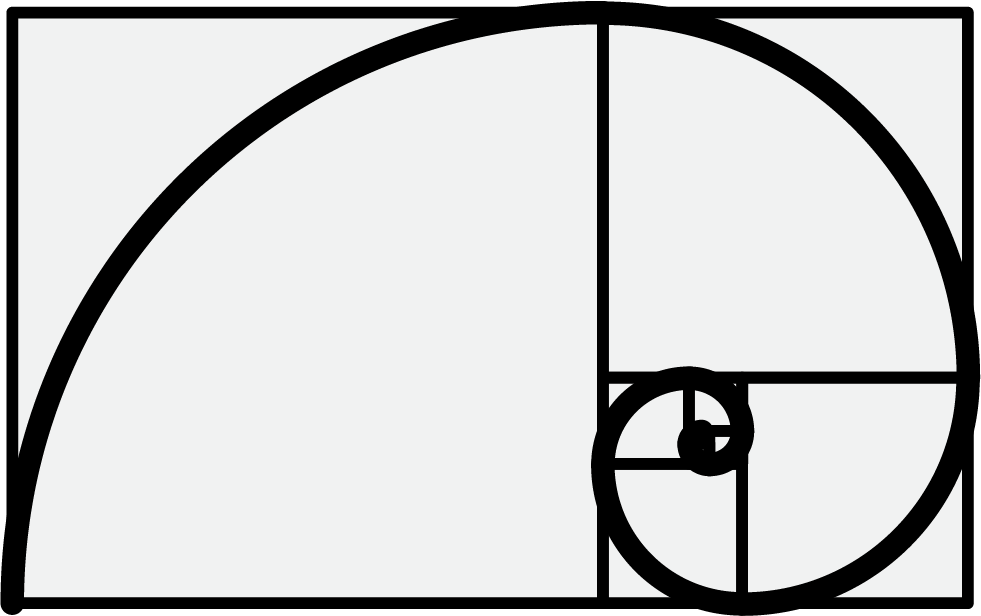
\includegraphics[height=0.75cm]{../../AAA_template_latex_settings/pwr-control_logo_doc.png}}
\lfoot{\href{http://www.pwr-control.com}{pwr-control.com}}
\cfoot{-\ \thepage\ -}
\rfoot{\textit{}}
\renewcommand{\headrulewidth}{0.4pt}
\renewcommand{\footrulewidth}{0.4pt}


\geometry{
	a4paper,
	top    = 2.5cm,
	bottom = 3.0cm,
	left   = 2.5cm,
	right  = 2.5cm
}

\hypersetup{
	colorlinks = true,
	urlcolor   = blue,
	linkcolor  = black,
	citecolor  = black
}

\pagenumbering{gobble}

% =============================================================
%  DOCUMENT METADATA
% =============================================================

\newcommand{\DocCategory}{Technical Research Report}
\newcommand{\DocField}{Power Electronics and Control Systems}

\newcommand{\DocTitle}{%
	{\fontsize{20}{24}\selectfont\bfseries Three Phase Inductors:} \\[16pt]
	{\fontsize{16}{20}\selectfont\bfseries mathematical model, construction and saturation effects.}
}

\newcommand{\DocSubtitle}{%
	Differential and common mode inductance of three-phase reactors.
}

\newcommand{\DocAuthor}{Davide Bagnara}
\newcommand{\DocRevision}{00}
\newcommand{\DocDate}{September 2024}

\newcommand{\DocAbstract}{%
	A three-phase inductor is not fully described by a single inductance value: the way the three windings share the magnetic circuit decides how the component reacts to differential mode currents and to common mode currents, and the two behaviours may differ by orders of magnitude. This note derives the corresponding model. Starting from the voltage equations of three coupled windings, written in terms of the self inductance $L_a$ and of the mutual inductance $L_m$, a transformation into phase-to-phase and zero sequence quantities decouples the system into a differential mode (positive sequence) inductance $L_p = L_a + L_m$ and a common mode (zero sequence) inductance $L_0 = L_a - 2L_m$, together with the relations which convert one set of parameters into the other. The three usual constructions are then read through the model: the four limb core, which carries both modes, the three limb core, which is essentially a differential mode reactor whose residual common mode inductance is the leakage, and the single limb or toroidal core used for common mode chokes. The last section extends the model to saturation, making $L_a$ and $L_m$ depend on the phase currents through a saturation factor which degrades them down to their air values $L_{a0}$ and $L_{m0}$, the condition reached for instance during a short circuit, and gives the resulting current dependent inductance matrix.
}

% Righe della revision history: Rev. & Date & Description & Authors \\
\newcommand{\RevisionHistory}{%
	00 & September 2024 & First issue. & \DocAuthor \\
}

% Metadati in fondo al frontespizio
\newcommand{\MetaLabelA}{Project Repository}
\newcommand{\MetaValueAUrl}{https://github.com/pwr-control/modelization-and-control.git}
\newcommand{\MetaValueALabel}{modelization-and-control.git}

\newcommand{\MetaLabelB}{Framework}
\newcommand{\MetaValueB}{MATLAB/Simulink/Simscape}

% =============================================================
%  DOCUMENTO
% =============================================================
\begin{document}
	% =============================================================
%  pwr-control LaTeX template - FRONTESPIZIO
%
%  Da richiamare come prima istruzione dopo \begin{document}:
%      % =============================================================
%  pwr-control LaTeX template - FRONTESPIZIO
%
%  Da richiamare come prima istruzione dopo \begin{document}:
%      % =============================================================
%  pwr-control LaTeX template - FRONTESPIZIO
%
%  Da richiamare come prima istruzione dopo \begin{document}:
%      \input{../../AAA_template_latex_settings/titlepage}
%
%  Il documento deve definire prima di \begin{document}:
%      \DocCategory   categoria del documento
%      \DocField      area tecnica
%      \DocTitle      titolo (una o due righe)
%      \DocSubtitle   sottotitolo
%      \DocAuthor     autore/i, separati da virgola
%      \DocRevision   numero di revisione corrente (es. 00)
%      \DocDate       data della revisione corrente
%      \DocAbstract   abstract
%      \RevisionHistory  righe della tabella di revisione, nel formato
%                        Rev. & Date & Description & Authors \\
%      \MetaLabelA \MetaValueAUrl \MetaValueALabel
%      \MetaLabelB \MetaValueB
% =============================================================

\providecommand{\DocCategory}{Technical Research Report}
\providecommand{\DocField}{Power Electronics and Control Systems}
\providecommand{\DocSubtitle}{}
\providecommand{\DocRevision}{00}
\providecommand{\DocAbstract}{}
\providecommand{\RevisionHistory}{%
	\DocRevision & \DocDate & First issue. & \DocAuthor \\
}

\titlepage

% ---- Intestazione centrata ----
\begin{center}
	{\Large\scshape \DocCategory}\\[8pt]
	{\large\scshape \DocField}
\end{center}

\vspace{30pt plus 4pt minus 14pt}
\noindent\rule{\linewidth}{0.8pt}

% ---- Titolo ----
\begin{center}
	\DocTitle
\end{center}

\vspace{4pt}
\noindent\rule{\linewidth}{2.2pt}

% ---- Sottotitolo ----
\begin{center}
	\begin{onehalfspace}
		{\large\itshape \DocSubtitle}
	\end{onehalfspace}
\end{center}

% ---- Authors / Revision / Date ----
\vspace{30pt plus 4pt minus 14pt}

\noindent
\begin{minipage}[t]{0.46\linewidth}
	\raggedright
	\textbf{Authors:}\\[2pt]
	\DocAuthor
\end{minipage}%
\hfill
\begin{minipage}[t]{0.22\linewidth}
	\centering
	\textbf{Revision:}\\[2pt]
	\DocRevision
\end{minipage}%
\hfill
\begin{minipage}[t]{0.30\linewidth}
	\raggedleft
	\textbf{Date:}\\[2pt]
	\DocDate
\end{minipage}

\vspace{10pt}
\noindent\rule{\linewidth}{0.8pt}

% ---- Abstract ----
\vspace{24pt plus 4pt minus 12pt}

\begin{center}
	\begin{minipage}{0.88\linewidth}
		\footnotesize
		\begin{onehalfspace}
			\textbf{Abstract:} \DocAbstract
		\end{onehalfspace}
	\end{minipage}
\end{center}

\vfill

% ---- Revision history ----
\begin{center}
	\begin{minipage}{0.96\linewidth}
		\centering
		{\footnotesize\scshape Revision history}\\[6pt]
		{\footnotesize
			\begin{tabular}{@{}cl>{\raggedright\arraybackslash}p{0.36\linewidth}>{\raggedright\arraybackslash}p{0.28\linewidth}@{}}
				\toprule
				\textbf{Rev.} & \textbf{Date} & \textbf{Description} & \textbf{Authors} \\
				\midrule
				\RevisionHistory
				\bottomrule
			\end{tabular}}
	\end{minipage}
\end{center}

\vspace{18pt plus 4pt minus 10pt}

% ---- Metadati in fondo ----
\noindent
\begin{tabular}{@{} r @{\quad} l @{}}
	\textsc{\MetaLabelA:} & {\href{\MetaValueAUrl}{\MetaValueALabel}} \\[3pt]
	\textsc{\MetaLabelB:} & {\MetaValueB}       \\[3pt]
\end{tabular}

% =============================================================
%  Fine frontespizio
% =============================================================
\newpage
\pagenumbering{arabic}
\setcounter{page}{1}

%
%  Il documento deve definire prima di \begin{document}:
%      \DocCategory   categoria del documento
%      \DocField      area tecnica
%      \DocTitle      titolo (una o due righe)
%      \DocSubtitle   sottotitolo
%      \DocAuthor     autore/i, separati da virgola
%      \DocRevision   numero di revisione corrente (es. 00)
%      \DocDate       data della revisione corrente
%      \DocAbstract   abstract
%      \RevisionHistory  righe della tabella di revisione, nel formato
%                        Rev. & Date & Description & Authors \\
%      \MetaLabelA \MetaValueAUrl \MetaValueALabel
%      \MetaLabelB \MetaValueB
% =============================================================

\providecommand{\DocCategory}{Technical Research Report}
\providecommand{\DocField}{Power Electronics and Control Systems}
\providecommand{\DocSubtitle}{}
\providecommand{\DocRevision}{00}
\providecommand{\DocAbstract}{}
\providecommand{\RevisionHistory}{%
	\DocRevision & \DocDate & First issue. & \DocAuthor \\
}

\titlepage

% ---- Intestazione centrata ----
\begin{center}
	{\Large\scshape \DocCategory}\\[8pt]
	{\large\scshape \DocField}
\end{center}

\vspace{30pt plus 4pt minus 14pt}
\noindent\rule{\linewidth}{0.8pt}

% ---- Titolo ----
\begin{center}
	\DocTitle
\end{center}

\vspace{4pt}
\noindent\rule{\linewidth}{2.2pt}

% ---- Sottotitolo ----
\begin{center}
	\begin{onehalfspace}
		{\large\itshape \DocSubtitle}
	\end{onehalfspace}
\end{center}

% ---- Authors / Revision / Date ----
\vspace{30pt plus 4pt minus 14pt}

\noindent
\begin{minipage}[t]{0.46\linewidth}
	\raggedright
	\textbf{Authors:}\\[2pt]
	\DocAuthor
\end{minipage}%
\hfill
\begin{minipage}[t]{0.22\linewidth}
	\centering
	\textbf{Revision:}\\[2pt]
	\DocRevision
\end{minipage}%
\hfill
\begin{minipage}[t]{0.30\linewidth}
	\raggedleft
	\textbf{Date:}\\[2pt]
	\DocDate
\end{minipage}

\vspace{10pt}
\noindent\rule{\linewidth}{0.8pt}

% ---- Abstract ----
\vspace{24pt plus 4pt minus 12pt}

\begin{center}
	\begin{minipage}{0.88\linewidth}
		\footnotesize
		\begin{onehalfspace}
			\textbf{Abstract:} \DocAbstract
		\end{onehalfspace}
	\end{minipage}
\end{center}

\vfill

% ---- Revision history ----
\begin{center}
	\begin{minipage}{0.96\linewidth}
		\centering
		{\footnotesize\scshape Revision history}\\[6pt]
		{\footnotesize
			\begin{tabular}{@{}cl>{\raggedright\arraybackslash}p{0.36\linewidth}>{\raggedright\arraybackslash}p{0.28\linewidth}@{}}
				\toprule
				\textbf{Rev.} & \textbf{Date} & \textbf{Description} & \textbf{Authors} \\
				\midrule
				\RevisionHistory
				\bottomrule
			\end{tabular}}
	\end{minipage}
\end{center}

\vspace{18pt plus 4pt minus 10pt}

% ---- Metadati in fondo ----
\noindent
\begin{tabular}{@{} r @{\quad} l @{}}
	\textsc{\MetaLabelA:} & {\href{\MetaValueAUrl}{\MetaValueALabel}} \\[3pt]
	\textsc{\MetaLabelB:} & {\MetaValueB}       \\[3pt]
\end{tabular}

% =============================================================
%  Fine frontespizio
% =============================================================
\newpage
\pagenumbering{arabic}
\setcounter{page}{1}

%
%  Il documento deve definire prima di \begin{document}:
%      \DocCategory   categoria del documento
%      \DocField      area tecnica
%      \DocTitle      titolo (una o due righe)
%      \DocSubtitle   sottotitolo
%      \DocAuthor     autore/i, separati da virgola
%      \DocRevision   numero di revisione corrente (es. 00)
%      \DocDate       data della revisione corrente
%      \DocAbstract   abstract
%      \RevisionHistory  righe della tabella di revisione, nel formato
%                        Rev. & Date & Description & Authors \\
%      \MetaLabelA \MetaValueAUrl \MetaValueALabel
%      \MetaLabelB \MetaValueB
% =============================================================

\providecommand{\DocCategory}{Technical Research Report}
\providecommand{\DocField}{Power Electronics and Control Systems}
\providecommand{\DocSubtitle}{}
\providecommand{\DocRevision}{00}
\providecommand{\DocAbstract}{}
\providecommand{\RevisionHistory}{%
	\DocRevision & \DocDate & First issue. & \DocAuthor \\
}

\titlepage

% ---- Intestazione centrata ----
\begin{center}
	{\Large\scshape \DocCategory}\\[8pt]
	{\large\scshape \DocField}
\end{center}

\vspace{30pt plus 4pt minus 14pt}
\noindent\rule{\linewidth}{0.8pt}

% ---- Titolo ----
\begin{center}
	\DocTitle
\end{center}

\vspace{4pt}
\noindent\rule{\linewidth}{2.2pt}

% ---- Sottotitolo ----
\begin{center}
	\begin{onehalfspace}
		{\large\itshape \DocSubtitle}
	\end{onehalfspace}
\end{center}

% ---- Authors / Revision / Date ----
\vspace{30pt plus 4pt minus 14pt}

\noindent
\begin{minipage}[t]{0.46\linewidth}
	\raggedright
	\textbf{Authors:}\\[2pt]
	\DocAuthor
\end{minipage}%
\hfill
\begin{minipage}[t]{0.22\linewidth}
	\centering
	\textbf{Revision:}\\[2pt]
	\DocRevision
\end{minipage}%
\hfill
\begin{minipage}[t]{0.30\linewidth}
	\raggedleft
	\textbf{Date:}\\[2pt]
	\DocDate
\end{minipage}

\vspace{10pt}
\noindent\rule{\linewidth}{0.8pt}

% ---- Abstract ----
\vspace{24pt plus 4pt minus 12pt}

\begin{center}
	\begin{minipage}{0.88\linewidth}
		\footnotesize
		\begin{onehalfspace}
			\textbf{Abstract:} \DocAbstract
		\end{onehalfspace}
	\end{minipage}
\end{center}

\vfill

% ---- Revision history ----
\begin{center}
	\begin{minipage}{0.96\linewidth}
		\centering
		{\footnotesize\scshape Revision history}\\[6pt]
		{\footnotesize
			\begin{tabular}{@{}cl>{\raggedright\arraybackslash}p{0.36\linewidth}>{\raggedright\arraybackslash}p{0.28\linewidth}@{}}
				\toprule
				\textbf{Rev.} & \textbf{Date} & \textbf{Description} & \textbf{Authors} \\
				\midrule
				\RevisionHistory
				\bottomrule
			\end{tabular}}
	\end{minipage}
\end{center}

\vspace{18pt plus 4pt minus 10pt}

% ---- Metadati in fondo ----
\noindent
\begin{tabular}{@{} r @{\quad} l @{}}
	\textsc{\MetaLabelA:} & {\href{\MetaValueAUrl}{\MetaValueALabel}} \\[3pt]
	\textsc{\MetaLabelB:} & {\MetaValueB}       \\[3pt]
\end{tabular}

% =============================================================
%  Fine frontespizio
% =============================================================
\newpage
\pagenumbering{arabic}
\setcounter{page}{1}

	\tableofcontents
	\listoffigures
	\listoftables
	\newpage

\begin{onehalfspace}

	\pagebreak
	\section{Three phase inductance: mathematical model}
	\noindent\textbf{Three-phase inductance with four limbs}:
	\begin{figure}[H]
		\centering
		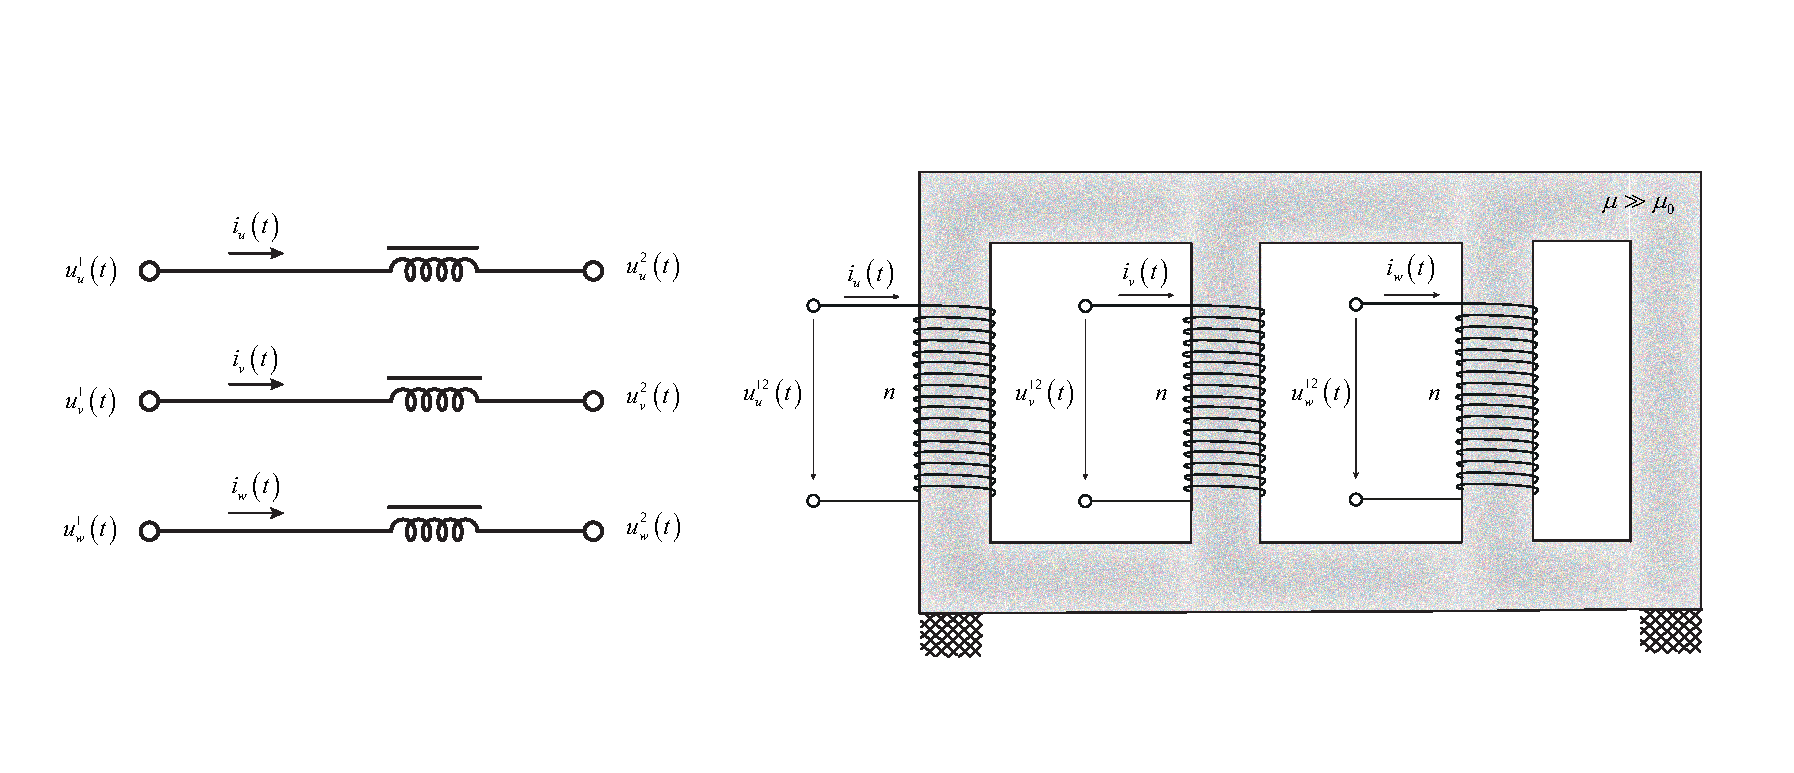
\includegraphics[width = 500pt, angle = 0, 
		keepaspectratio]{figures/three-phase-inductor-ver-i.eps}
		\captionsetup{width=0.75\textwidth, font=small}	
		\caption{Three-phase inductance: differential and common operational mode with four magnetic limbs.}
		\label{fig1}
	\end{figure}
	\noindent\textbf{Three-phase inductance with three limbs - pure differential mode}:
	\begin{figure}[H]
		\centering
		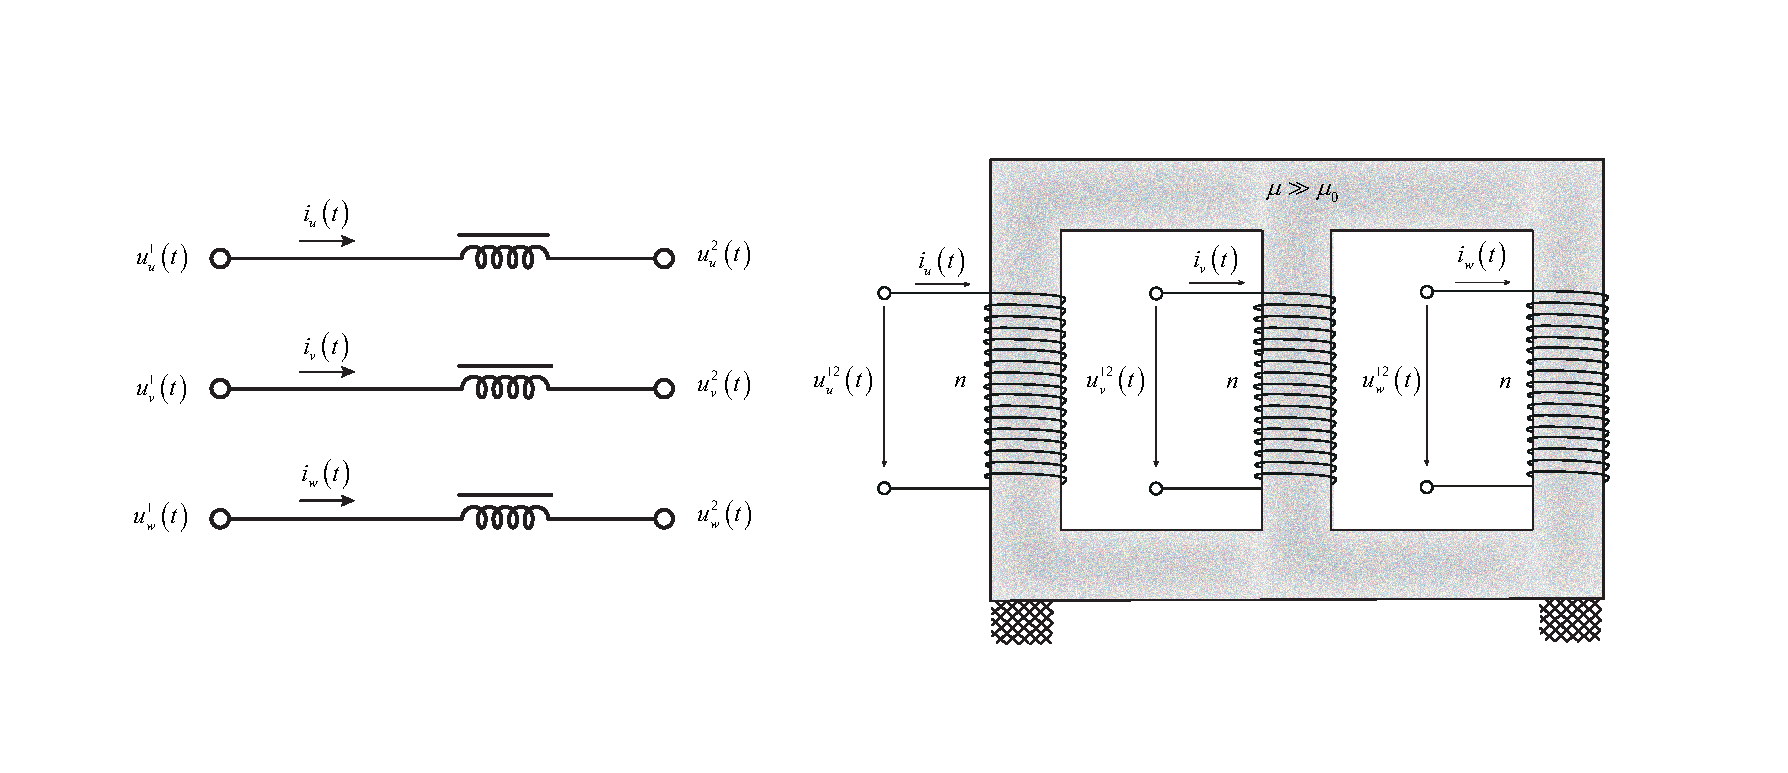
\includegraphics[width = 500pt, angle = 0, 
		keepaspectratio]{figures/three-phase-inductor-dm-ver-i.eps}
		\captionsetup{width=0.75\textwidth, font=small}	
		\caption{Three-phase inductance: pure differential operative mode with three magnetic limbs.}
		\label{fig2}
	\end{figure}
	
	\noindent\textbf{Three-phase inductance with one limb - pure common mode}:
	\begin{figure}[H]
		\centering
		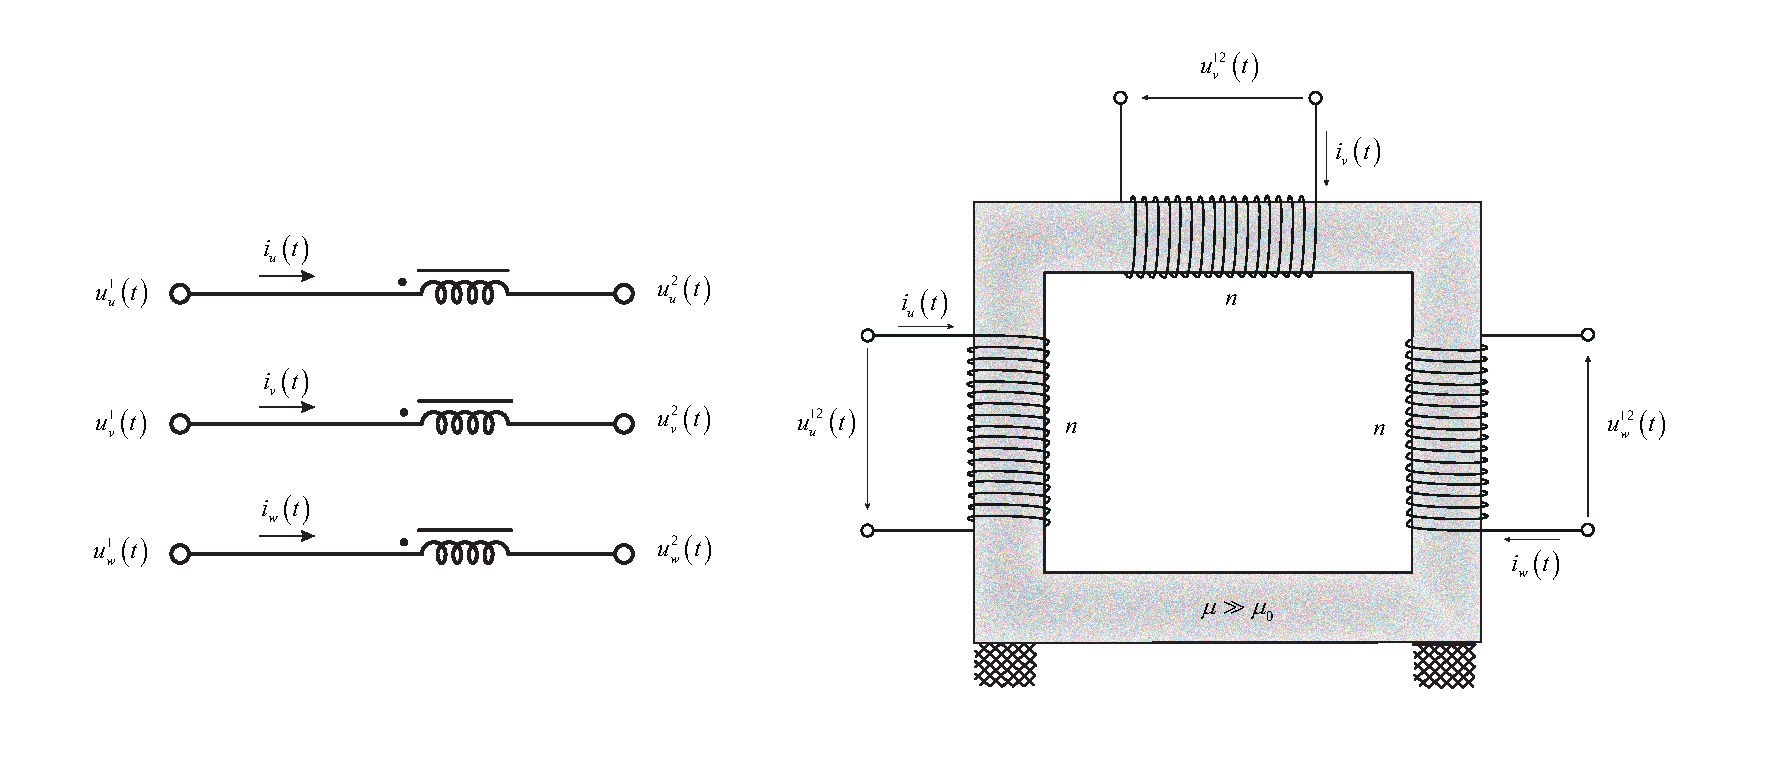
\includegraphics[width = 500pt, angle = 0, 
		keepaspectratio]{figures/three-phase-inductor-cm-ver-i.eps}
		\captionsetup{width=0.75\textwidth, font=small}	
		\caption{Three-phase inductance: pure common operative mode with one magnetic limbs (classical toroidal core is used for low power application).}
		\label{fig3}
	\end{figure}
	\noindent\textbf{Mathematical model}:
	\begin{equation}\left\lbrace 
		\begin{aligned}
			u_u^{12}(t) &= u_u^{cm}(t)+u_u^{dm}(t) \\[6pt]
			u_v^{12}(t) &= u_v^{cm}(t)+u_v^{dm}(t) \\[6pt]
			u_w^{12}(t) &= u_w^{cm}(t)+u_w^{dm}(t) \\[6pt]
		\end{aligned}\right. 
	\end{equation}
	where
	\begin{equation}\left\lbrace 
		\begin{aligned}
			u_u^{dm}(t) + u_v^{dm}(t) + u_w^{dm}(t) &= 0 \\[6pt]
			\frac{1}{3}\Big(u_u^{cm}(t) + u_v^{cm}(t) + u_w^{cm}(t)\Big) &= u_{cm}(t) \\[6pt]
		\end{aligned}\right. 
	\end{equation}
	
	\begin{equation}\left\lbrace 
		\begin{aligned}
			u_u^{12}(t) -R i_u(t) - L_a \frac{d\,i_u}{dt}(t) + L_m \frac{d\,i_v}{dt}(t) + L_m \frac{d\,i_w}{dt}(t) &= 0 \\[6pt]
			u_v^{12}(t) -R i_v(t) - L_a \frac{d\,i_v}{dt}(t) + L_m \frac{d\,i_u}{dt}(t) + L_m \frac{d\,i_w}{dt}(t) &= 0 \\[6pt]
			u_w^{12}(t) -R i_w(t) - L_a \frac{d\,i_w}{dt}(t) + L_m \frac{d\,i_u}{dt}(t) + L_m \frac{d\,i_v}{dt}(t) &= 0 \\[6pt]
		\end{aligned}\right. 
	\end{equation}
	which results in matrix form
	\begin{equation}
		\vec{u}_{uvw}^{12}(t) - \mathbf{R}\vec{i}_{uvw}(t) - \mathbf{L}\frac{d}{dt}\vec{i}_{uvw}(t) = 0
	\end{equation}
	where
	\begin{equation}
		\mathbf{R} = \begin{bmatrix} R & 0 & 0 \\ 0 & R & 0 \\ 0 & 0 & R \end{bmatrix}, \qquad 
		\mathbf{L} = \begin{bmatrix} L_a & -L_m & -L_m \\ -L_m & L_a & -L_m \\ -L_m & -L_m & L_a \end{bmatrix}.
	\end{equation}
	in order to derive the equivalent \textit{differential} and \textit{common} mode equations the following transformation matrix is accounted
	\begin{equation}
		\mathbf{T} = \begin{bmatrix} 1 & -1 & 0 \\ 0 & 1 & -1 \\ -1 & 0 & 1 \\ \frac{1}{3} & \frac{1}{3} & \frac{1}{3} \end{bmatrix}.
	\end{equation}
	where
	\begin{equation}
		\vec{u}_{uvw}^{12} = \begin{bmatrix} u^{12}_{u}(t) \\[6pt] u^{12}_{v}(t) \\[6pt] u^{12}_{w}(t) \end{bmatrix}= \mathbf{T}^{-1}\begin{bmatrix} u^{dm}_{uv}(t) \\[6pt] u^{dm}_{vw}(t) \\[6pt] u^{dm}_{wu}(t) \\[6pt] u_{cm}(t) \end{bmatrix}.
	\end{equation}
	where
	\begin{equation}
		\begin{bmatrix} u^{dm}_{uv}(t) \\[6pt] u^{dm}_{vw}(t) \\[6pt] u^{dm}_{wu}(t) \\[6pt] u_{cm}(t) \end{bmatrix} - \begin{bmatrix} R & -R & 0 \\ 0 & R & -R \\ -R & 0 & R \\ R & R & R \end{bmatrix} \begin{bmatrix} i_u(t) \\ i_v(t) \\ i_w(t) \end{bmatrix} - \begin{bmatrix} L_a+L_m & -(L_a+L_m) & 0 \\ 0 & L_a+L_m & -(L_a+L_m) \\ -(L_a+L_m) & 0 & L_a+L_m \\ L_a-2L_m & L_a-2L_m & L_a-2L_m \end{bmatrix} \begin{bmatrix} \frac{di_u}{dt}(t) \\ \frac{di_v}{dt}(t) \\ \frac{di_w}{dt}(t) \end{bmatrix} = 0
	\end{equation}
	expressing in terms of $\begin{bmatrix} u^{12}_{dmu}(t) & u^{12}_{dmv}(t) & u^{12}_{dmu}(t) \end{bmatrix}^{T}$ and $u_{cm}(t)$ we obtain the following system
	
	\begin{equation}
		\vec{u}_{duvw}^{12}(t) - \mathbf{R}\vec{i}_{uvw}(t) - \mathbf{L}_{dm}\frac{d}{dt}\vec{i}_{uvw}(t) = 0
	\end{equation}
	where
	\begin{equation}
		\mathbf{R} = \begin{bmatrix} R & 0 & 0 \\ 0 & R & 0 \\ 0 & 0 & R \end{bmatrix}, \qquad 
		\mathbf{L} = \begin{bmatrix} L_a+L_m & 0 & 0 \\ 0 & L_a+L_m & 0 \\ 0 & 0 & L_a+L_m \end{bmatrix}.
	\end{equation}
	and 
	\begin{equation}
		{u}_{cm}(t) - R {i}_{cm}(t) - (L_a-2L_m)\frac{d}{dt}{i}_{cm}(t) = 0
	\end{equation}
	where ${i}_{cm}(t) = \frac{1}{3}\Big(i_u(t)+i_v(t)+i_w(t)\Big)$.
	Hence, in a three-phase inductance we have two inductive contributions
	\begin{itemize}
		\item[--] differential mode (also called \textit{positive sequence inductance}) given by $L_p = L_a + L_m$;
		\item[--] common mode (also called \textit{zero sequence inductance}) given by $L_0 = L_a -2L_m$
	\end{itemize}
	where $L_a$ is the self-inductance, and $L_m$ is the mutual-inductance.
	
	The relation between sequence values and machine values can be summarized as follows
	\begin{equation}\left\lbrace 
		\begin{aligned}
			L_p &= L_a + L_m \\[6pt]
			L_0 &= L_a -2L_m  \\[6pt]
			L_m &= \frac{1}{3}\Big(L_p - L_0\Big) \\[6pt]
			L_a &= \frac{1}{2}\Big(L_p + L_0 + L_m\Big) \\[6pt]
		\end{aligned}\right. 
	\end{equation}
	
	Commercially speaking three-phase inductor can be either \textit{common mode} or \textit{differential mode}:
	\begin{itemize}
		\item[--] Typically three-phase three-limbs inductors present only differential inductance. The residual common mode inductance is associated to the leakage inductance, see Figure~\ref{fig2}.
		\item[--] Typically three-phase common mode inductors are built around a common single limb core. The residual differential mode inductance is associated to the leakage inductance, see Figure~\ref{fig3}.
	\end{itemize}
	
	\section{Saturation effects}
	The saturation effects can be modelized assuming $L_a$ and $L_m$ as function of the current, as follows
	\begin{equation}\left\lbrace 
		\begin{aligned}
			L_{au} &= L_a^{nom} k_{sat}^{a}(i_u) + L_{a0}\rightarrow L_{a0}\quad\text{for } i\gg i_{sat}  \\[6pt]
			L_{av} &= L_a^{nom} k_{sat}^{a}(i_v) + L_{a0}\rightarrow L_{a0}\quad\text{for } i\gg i_{sat}  \\[6pt]
			L_{aw} &= L_a^{nom} k_{sat}^{a}(i_w) + L_{a0}\rightarrow L_{a0}\quad\text{for } i\gg i_{sat}  \\[6pt]
			L_{mu} &= L_m^{nom} k_{sat}^{m}(i_u) + L_{m0}\rightarrow L_{m0}\quad\text{for } i\gg i_{sat}  \\[6pt]
			L_{mv} &= L_m^{nom} k_{sat}^{m}(i_v) + L_{m0}\rightarrow L_{m0}\quad\text{for } i\gg i_{sat}  \\[6pt]
			L_{mw} &= L_m^{nom} k_{sat}^{m}(i_w) + L_{m0}\rightarrow L_{m0}\quad\text{for } i\gg i_{sat}  \\[6pt]
		\end{aligned}\right. 
	\end{equation}
	where $L_{a0}$ and $L_{m0}$ are the equivalent self and mutual inductance in air, condition which raises e.g. during short circuit current. 
	\begin{figure}[H]
		\centering
		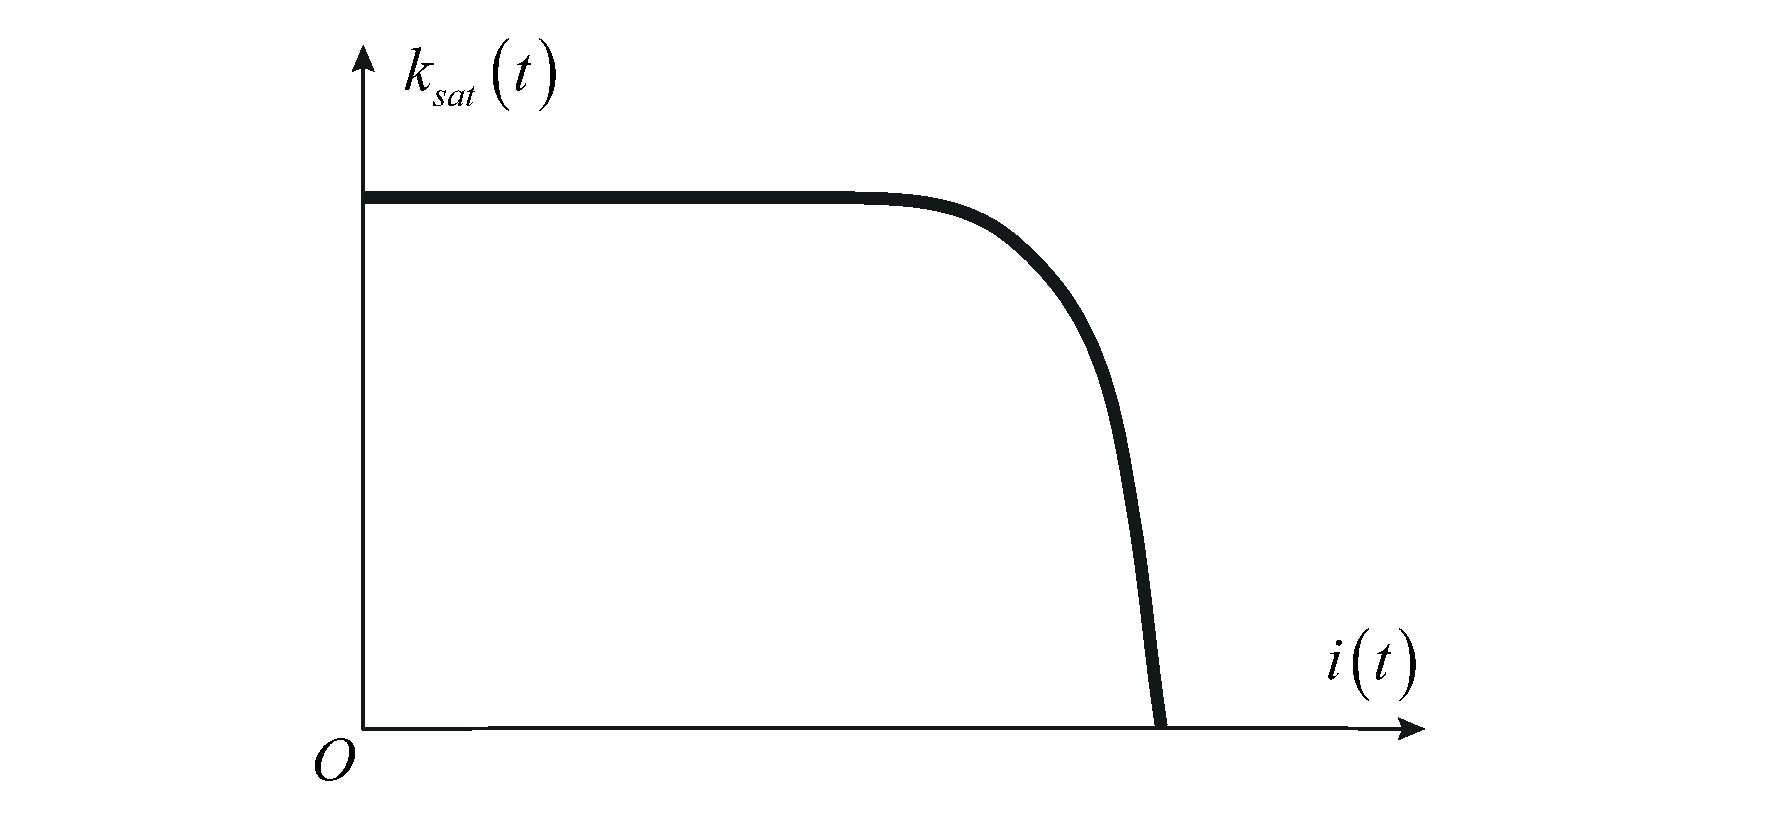
\includegraphics[width = 300pt, angle = 0, 
		keepaspectratio]{figures/saturation-curve-ver-i.eps}
		\captionsetup{width=0.75\textwidth, font=small}	
		\caption{Saturation curve applied to $L_a$ and $L_m$, self and mutual inductance respectively.}
		\label{fig4}
	\end{figure}
	
	
	\begin{equation}
		\mathbf{L}(\vec{i}_{uvw}) = \begin{bmatrix} L_{ls}+L_a^{nom} k_{sat}^{a}(i_u) + L_{a0} & -\big[L_m^{nom} k_{sat}^{m}(i_v) + L_{m0}\big] & -\big[L_m^{nom} k_{sat}^{m}(i_w) + L_{m0}\big] \\[6pt] -\big[L_m^{nom} k_{sat}^{m}(i_u) + L_{m0}\big] & L_{ls}+L_a^{nom} k_{sat}^{a}(i_v) + L_{a0} & -\big[L_m^{nom} k_{sat}^{m}(i_w) + L_{m0}\big] \\[6pt] -\big[L_m^{nom} k_{sat}^{m}(i_u) + L_{m0}\big] & -\big[L_m^{nom} k_{sat}^{m}(i_v) + L_{m0}\big] & L_{ls}+L_a^{nom} k_{sat}^{a}(i_w) + L_{a0} \end{bmatrix}
	\end{equation}
	
	\newpage
	\begin{thebibliography}{9}
		\bibitem{heldwein} 
		M. L. Heldwein, L. Dalessandro, J. W. Kolar - \emph{The Three-Phase Common-Mode Inductor: Modeling Design Issues}. IEEE Transactions on industrial electronics, vol. 58, no. 8, August 2011.
		\bibitem{Hurley} 
		W. G. Hurley, W. H. Woelfle - \emph{Transformers and Inductors for Power Electronics. Theory design and applications}. J. Wiley 2013.
	\end{thebibliography}
	
	%*********************************************************
	% Print bibliography (If bibliography is empty nothing happens)
	%*********************************************************
	%\newpage
	%\printbibliography[heading=bibintoc]
\end{onehalfspace}
\end{document} 